\documentclass{article}

% Lenguaje y Fuente
\usepackage[spanish]{babel}
\usepackage[utf8x]{inputenc}
\usepackage[T1]{fontenc}
\usepackage[top=1in, bottom=1.25in, left=1.1 in, right=1.1 in]{geometry}
\usepackage{graphicx}
\usepackage{ragged2e}
\usepackage[usenames]{color}
\usepackage{multicol}

% Portada

\title{\textbf{Reporte de la Actividad 8}\\ Uniendo DataFrames en Pandas}
\author{Luis Fernando Duarte Gonzalí \\ Universidad de Sonora \\ Física Computacional}
\date{Abril del 2019}
\begin{document}
\maketitle

% Contenido del Reporte

\section{Introducción}
En esta actividad trabajaremos con 2 conjuntos de datos: Los datos meteorológicos de la estación de Nogal que ya se trabajó en la actividad 7. El segundo conjunto de datos se refieren a datos del suelo. Ambos conjuntos de datos coinciden en el periodo 2009, que será el periodo que nos interesa estudiar. El segundo conjunto de datos son sobre variables medidas por sensores bajo el suelo, gestionados y almacenados por un segundo data logger. 

Nos interesa crear en los datos del suelo una nueva columna con una variable temporal similar a la que se tiene en los datos meteorológicos, para poder incorporar un conjunto de variables nuevas. Las variables que nos interesan estudiar son los relacionados con las lecturas de temperatura del suelo Tsuelo\_10cm, Suelo\_20cm, ..., Tsuelo\_100cm en 8 profundidades distintas. Adicionalmente se desea incorporar la temperatura del aire del dataframe de datos meteorológicos.

\section{Análisis de Datos}
Primero tenemos que cargar a nuestro código las librerías que vamos a necesitar durante la actividad.
\begin{center}
    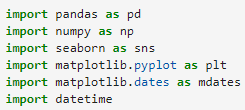
\includegraphics[scale = 0.7]{import.png}
\end{center}

Leemos el archivo de la manera que hemos estado usando:

\begin{center}
    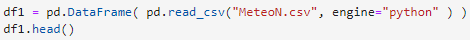
\includegraphics[scale = 0.7]{read1.png}
\end{center}

Se siguió el mismo procedimiento que en la actividad 7, pero como ahora uniremos ambos dataframes en uno, se creó un formato de fecha.
\\

Leemos el segundo archivo que vamos a utilizar:
\begin{center}
    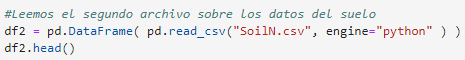
\includegraphics[scale = 0.7]{read2.png}
\end{center}
\clearpage

Filtramos los datos que nos interesan del segundo archivo
\begin{center}
    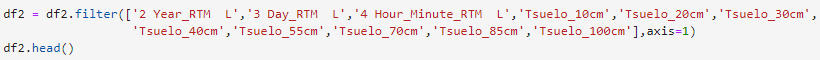
\includegraphics[scale = 0.7]{filtrar.png}
\end{center}
Creamos dos arreglos para separar las horas y minutos. Convertimos a tipo string la columna de minutos y horas.

\begin{center}
    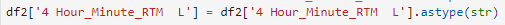
\includegraphics[scale = 0.7]{24h.png}
\end{center}
Extraemos las horas y minutos de esa columna por separado:
\begin{center}
    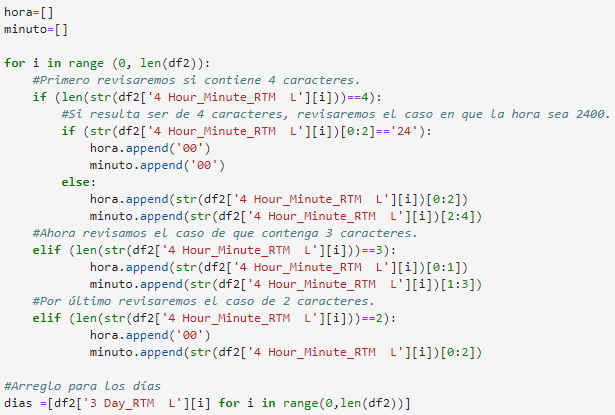
\includegraphics[scale = 0.7]{HrMin.png}
\end{center}

Creamos un DataFrame nuevo con los días, horas y minutos.

\begin{center}
    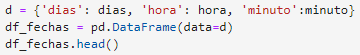
\includegraphics[scale = 0.7]{Dd.png}
\end{center}

Filtrados los datos, creando el formato de fecha, agregando un día cuando se marcaran las 0 horas, después se unieron ambos DataFrames en uno solo:
\begin{center}
    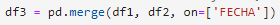
\includegraphics[scale = 0.7]{merge.png}
\end{center}

Después de todo eso, se empezaron a generar las gráficas que buscamos desde el principio para mostrar el análisis de datos completo.
\clearpage

\subsection{Resultados}
En las siguientes gráficas se muestran las temperaturas de un día (1 de Enero de 2009) del suelo y del aire.

\begin{center}
    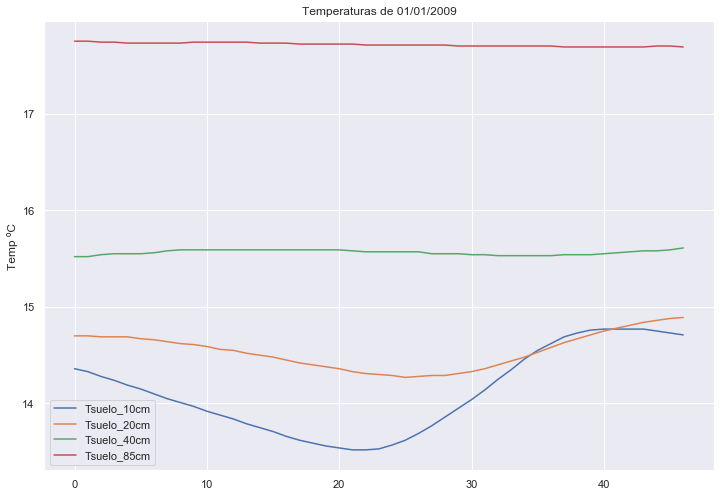
\includegraphics[scale = 0.3]{TGDay.png}
    \includegraphics[scale = 0.3]{TADay.png}
\end{center}

Temperaturas del suelo y del Aire.

\begin{center}
    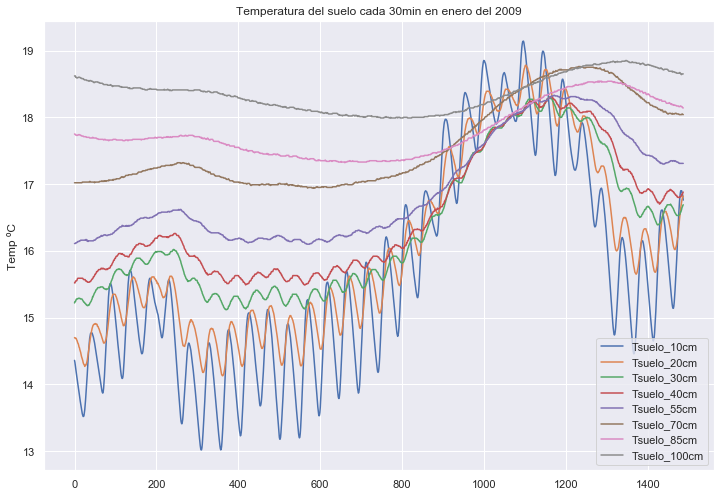
\includegraphics[scale = 0.3]{TG09.png}
    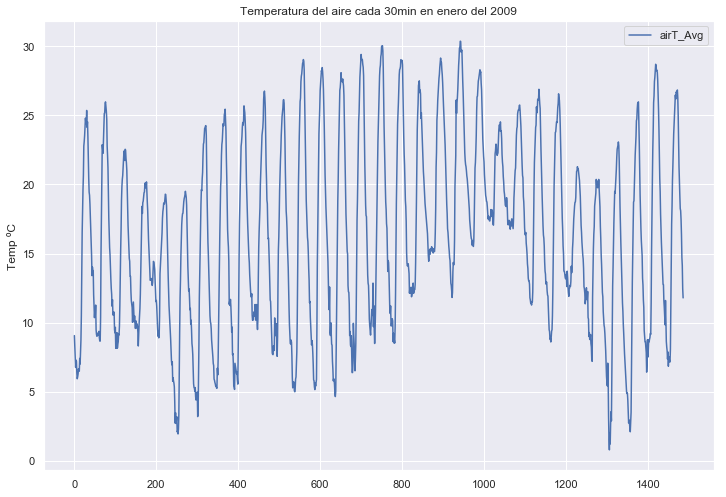
\includegraphics[scale = 0.3]{TA09.png}
\end{center}

En las gráficas que se muestran a continuación se muestra la temperatura del aire y del suelo en diferentes profundidades del mismo. A lado de cada gráfica se muestra las mismas gráficas usando el método de rolling mean, suavizando la evolución temporal de cada una.

\begin{center}
    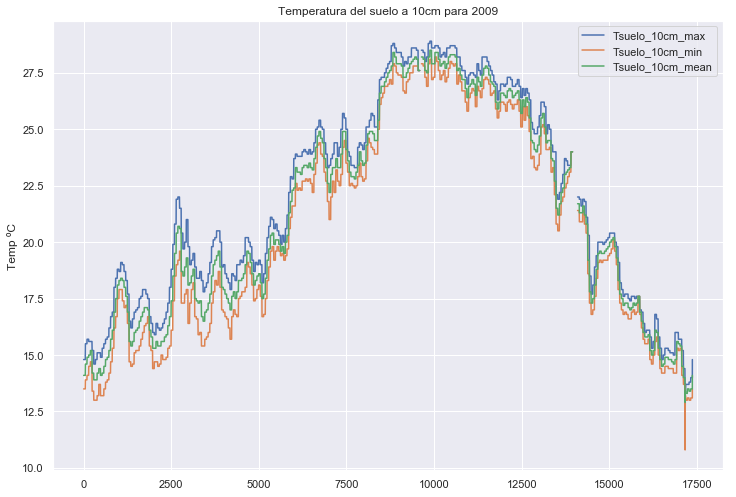
\includegraphics[scale = 0.3]{TG10.png}
    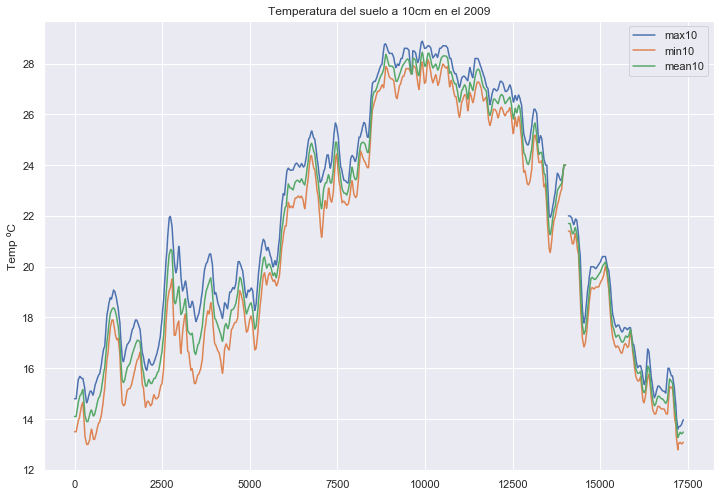
\includegraphics[scale = 0.3]{TG10S.png}
    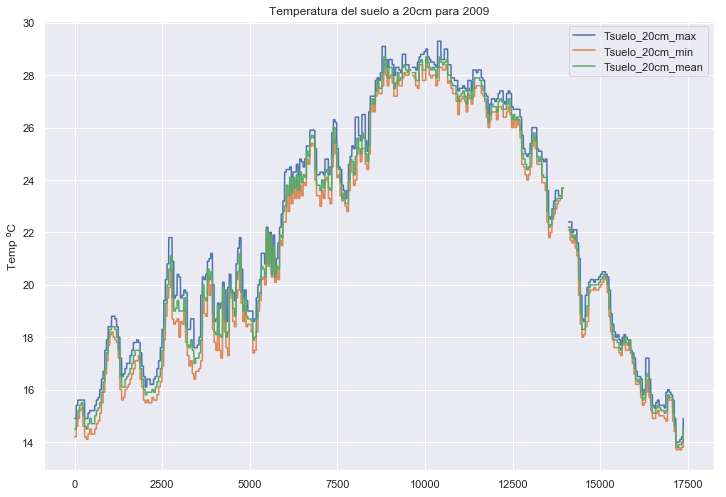
\includegraphics[scale = 0.3]{TG20.png}
    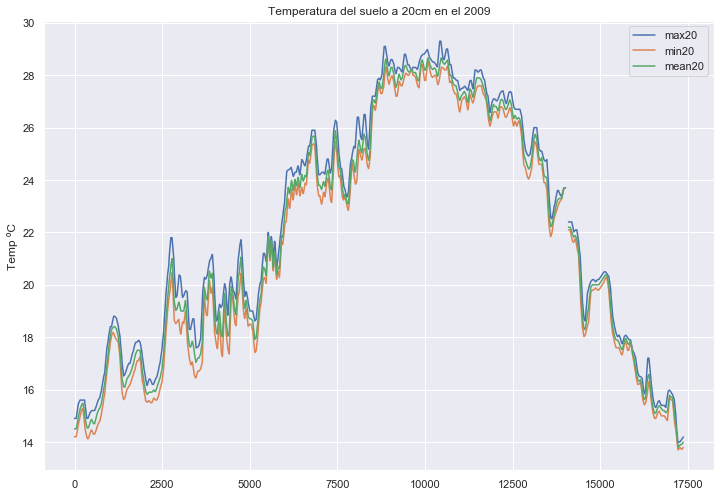
\includegraphics[scale = 0.3]{TG20S.png}
    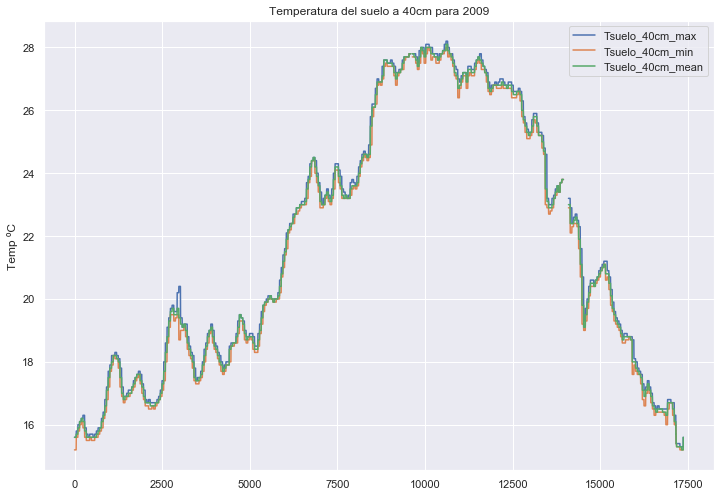
\includegraphics[scale = 0.3]{TG40.png}
    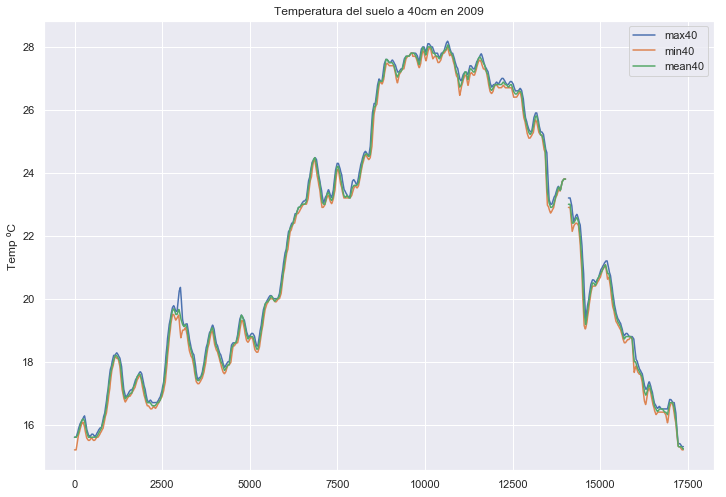
\includegraphics[scale = 0.3]{TG40S.png}
    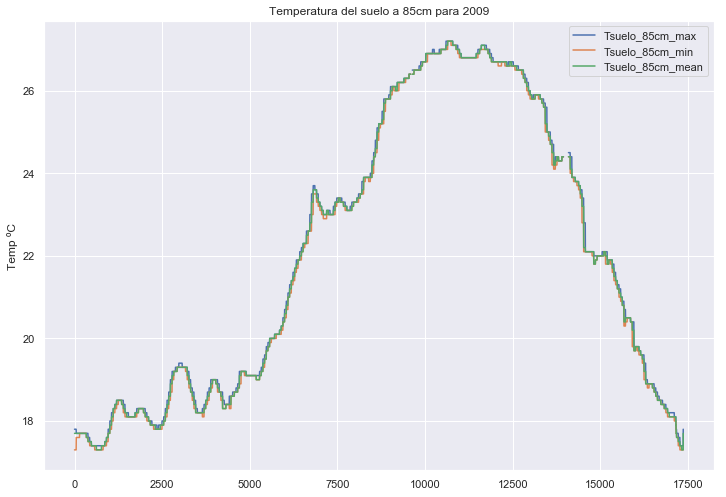
\includegraphics[scale = 0.3]{TG85.png}
    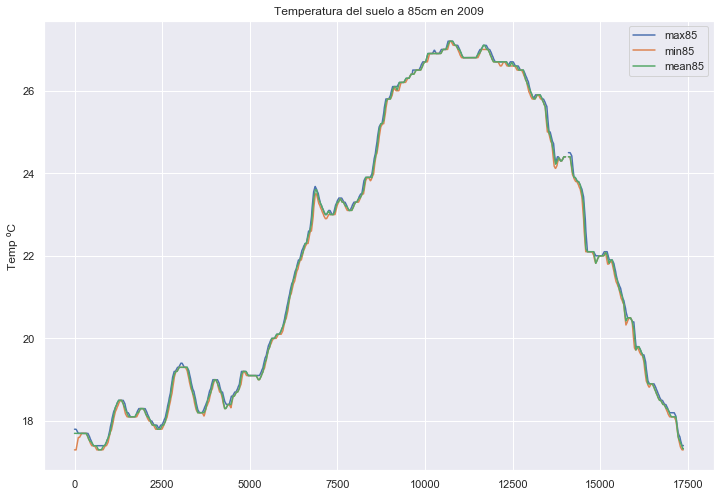
\includegraphics[scale = 0.3]{TG85S.png}
\end{center}

\section{Conclusión}
Al momento de observar las gráficas podemos notar el cambio de temperatura mientras más profundo en el suelo estamos, va de menor a mayor igual que la profundidad, además es más inestable en la superficie, mientras que a cierta distancia hay menos variaciones. Este efecto también se puede observar en las gráficas de cada 30 minutos, donde vemos que la temperatura es más caliente entre más profundo en el suelo estamos tomando las mediciones.

Al observar las gráficas de promedio, máximo y mínimo de temperaturas se hace evidente lo que se menciona anteriormente.

En sí la práctica tuvo su punto de mayor dificultad a la hora de combinar dos dataframes en uno para poder trabajar con sus datos en conjunto.

\section{Bibliografía}
\begin{itemize}
    \item Seaborn: statistical data visualization. (2018). Consultado en Abril del 2019, de Seaborn. Sitio web: 
    
    https://seaborn.pydata.org/
    
    \item Python Strings, Functions and Examples (2019). Consultado en Abril del 2019, de Tech Beamers Sitio web:
    
    https://www.techbeamers.com/python-strings-functions-and-examples/
    
    \item Merge, join, and concatenate. Consultado en Abril del 2019, de PandasPydata.org. Sitio web:
    
    https://pandas.pydata.org/pandas-docs/stable/user\_guide/merging.html
    
\end{itemize}



\end{document}
